\documentclass[tikz]{standalone}
\usepackage{stix}

\usetikzlibrary{matrix}

\newcommand{\dn}{{\color{red} $\uparrow$}}
\newcommand{\up}{$\downarrow$}

\begin{document}
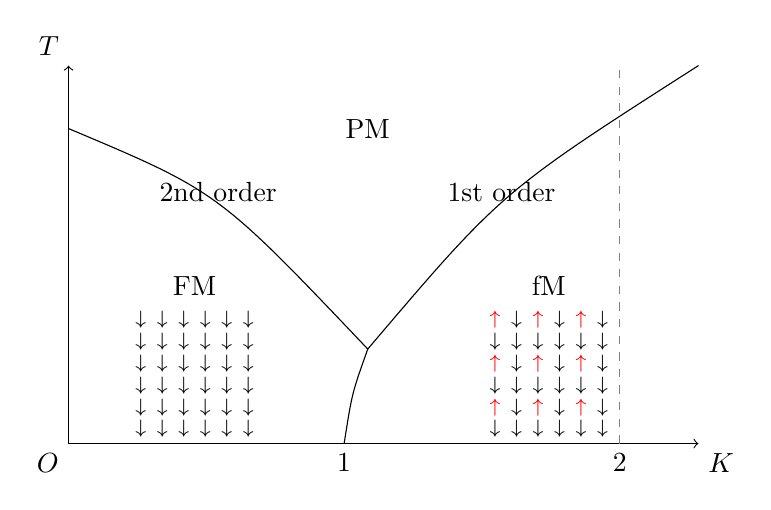
\begin{tikzpicture}[yscale=0.8]

\draw[->] node[anchor=north east] {$O$} (0,0) -- (8,0) node[anchor=north west] {$K$};
\draw[->] (0,0) -- (0,6) node[anchor=south east] {$T$};

\draw (3.5,0) .. controls (3.6,0.8) .. (3.8,1.5);
\draw (0,5) .. controls (1.9,4) .. (3.8,1.5);
\draw (3.8,1.5) .. controls (5.5,4) .. (8,6);
\draw[dashed,gray] (7,0) -- (7,6);

\node[anchor=north] at (3.5,0) {$1$};
\node[anchor=north] at (7,0) {$2$};
% \node[anchor=south west] at (0,5) {$A$};
% \node[anchor=south,yshift=8] at (3.8,1.5) {$B$};
% \node[anchor=north west] at (8,6) {$C$};
\node at (1.6,2.5) {FM};
\node at (6.1,2.5) {fM};
\node at (3.8,5) {PM};
\node at (1.9,4) {2nd order};
\node at (5.5,4) {1st order};

\matrix[matrix of nodes,anchor=north,font=\tt \scriptsize,row sep=-5,column sep=-3] at (1.6,2.4) {
\up & \up & \up & \up & \up & \up \\
\up & \up & \up & \up & \up & \up \\
\up & \up & \up & \up & \up & \up \\
\up & \up & \up & \up & \up & \up \\
\up & \up & \up & \up & \up & \up \\
\up & \up & \up & \up & \up & \up \\
};
\matrix[matrix of nodes,anchor=north,font=\tt \scriptsize,row sep=-5,column sep=-3] at (6.1,2.4) {
\dn & \up & \dn & \up & \dn & \up \\
\up & \up & \up & \up & \up & \up \\
\dn & \up & \dn & \up & \dn & \up \\
\up & \up & \up & \up & \up & \up \\
\dn & \up & \dn & \up & \dn & \up \\
\up & \up & \up & \up & \up & \up \\
};

\end{tikzpicture}
\end{document}
